\documentclass[../main.tex]{subfiles}
\begin{document}
\chapter{Rotating Reference Frames}
\begin{remark}[Recap]
  Recall from \cref{referenceFrames} that a reference frame is \textit{inertial} if any free particle (one experiencing no forces) has constant velocity in that reference frame.
\end{remark}
Rotating reference frames are important examples of \textbf{non-inertial reference frames}.
\section{Newton's Equations in a Rotating Frame}
Suppose we have an inertial frame with $S$ with Cartesian axes $\vec{e}_1, \vec{e}_2, \vec{e}_3$ and a rotating frame $S'$ with axes $\vec{e}_1', \vec{e}_2', \vec{e}_3'$.

From the perspective of the inertial frame, the $\vec{e}_i'$ axes rotate with angular velocity $\omega$ and so each axis obeys \cref{angularVelocityCross}, that is:
\[
  \dot{\vec{e}}_i' = \vec{\omega} \times \vec{e}_i'
\]
In the two frames, the position of a particle is, respectively:
\[
  \vec{x} = x_i \vec{e}_i = x_i' \vec{e}_i' \quad \text{(using $\Sigma$ convention)}
\]
\begin{remark}[Notation]
  We use the notation $\left(\deriv{\vec{x}}{t}\right)_S$ to mean the derivative of the Cartesian components in $S$, that is:
  \[
    \left(\deriv{\vec{x}}{t}\right)_S = \dot{x}_i \vec{e}_i
  \]
  and the notation $\left(\deriv{\vec{x}}{t}\right)_{s'}$ to mean the derivative of the components in $S'$, that is:
  \[
    \left(\deriv{\vec{x}}{t}\right)_{S'} = \dot{x}'_i \vec{e}_i'
  \]
\end{remark}
We want to know how the laws of physics appear in the rotating frame and we do this by relating the components of $\vec{x}$ in each frame and then applying Newton's equation to the inertial frame.

To relate the velocities, we can differentiate $\dot{\vec{x}}$ in two ways to yield:
\begin{align*}
  \dot{\vec{x}} &= \dot{x}_i \vec{e}_i \\
                &= \dot{x}_i' \vec{e}_i' + x_i' \dot{\vec{e}}_i' \\
                &= \dot{x}_i' \vec{e}_i' + x_i' (\vec{\omega} \times \vec{e}_i') \\
                &= \dot{x}_i' \vec{e}_i' + \vec{\omega} \times (x_i' \vec{e}_i') \\
                &= \left(\deriv{\vec{x}}{t}\right)_{S'} + \vec{\omega} \times \vec{x}
\end{align*}
Therefore, we have:
\[
  \left(\deriv{\vec{x}}{t}\right)_{S} = \left(\deriv{\vec{x}}{t}\right)_{S'} + \vec{\omega} \times \vec{x}
\]
This intuitively makes sense as we expect the velocity of the particle in the inertial frame to be the velocity of the particle in the non-inertial frame plus the velocity due to the rotation $\vec{\omega} \times \vec{x}$.

To use Newton's 2nd law we need the acceleration:
\begin{align*}
  \ddot{\vec{x}} &= \ddot{x}_i \vec{e}_i \\
                 &= \deriv{}{t}(\dot{x}_i' \vec{e}_i' + \vec{\omega} \times \vec{x}) \\
                 &= \ddot{x}_i' \vec{e}_i' + \dot{x}_i' \dot{\vec{e}}_i' + \dot{\vec{\omega}} \times \vec{x} + \vec{\omega} \times \dot{\vec{x}} \\
                 &= \left(\deriv[2]{\vec{x}}{t}\right)_{S'} + \dot{x}_i' (\vec{\omega} \times \vec{e}_i') + \dot{\vec{\omega}} \times \vec{x} + \vec{\omega} \times \left[\left(\deriv{\vec{x}}{t}\right)_{S'} + \vec{\omega} \times \vec{x}\right]\\
                 &= \left(\deriv[2]{\vec{x}}{t}\right)_{S'} + \vec{\omega} \times \left(\deriv{\vec{x}}{t}\right)_{S'} + \dot{\vec{\omega}} \times \vec{x} + \vec{\omega} \times \left(\deriv{\vec{x}}{t}\right)_{S'} + \vec{\omega} \times (\vec{\omega} \times \vec{x})
\end{align*}
and so:
\[
  \left(\deriv[2]{\vec{x}}{t}\right)_{S} = \left(\deriv[2]{\vec{x}}{t}\right)_{S'} + \dot{\vec{\omega}} \times \vec{x} + 2 \vec{\omega} \times \left(\deriv{\vec{x}}{t}\right)_{S'} + \vec{\omega} \times (\vec{\omega} \times \vec{x})
\]
This is the key relation between the acceleration in a rotating frame an in an inertial frame.

We can now apply Newton's 2nd law to the inertial frame, so suppose that:
\[
  m \left(\deriv[2]{\vec{x}}{t}\right) = \vec{F}
\]
Therefore, in the rotating frame:
\[
  m \left(\deriv[2]{\vec{x}}{t}\right)_{S'} = \vec{F} -\underbrace{m \dot{\vec{\omega}} \times \vec{x}}_{\text{Euler Force}} - \underbrace{2 m \vec{\omega} \times \left(\deriv{\vec{x}}{t}\right)_{S'}}_{\text{Coriolis Force}} - \underbrace{m \vec{\omega} \times (\vec{\omega} \times \vec{x})}_{\text{Centrifugal Force}}
\]
The \textit{Euler Force}, \textit{Coriolis Force}, and \textit{Centrifugal Force} are all ``\textit{fictitious forces}''.

A free particle (i.e. $\vec{F} = \vec{0}$) does not move in a straight line in the rotating frame due to these fictitious forces.

An important example of this is the rotation of the Earth:
\[
  \omega_{\text{Earth}} = \frac{2\pi}{\text{1 day}} \approx \qty{7e-5}{\second^{-1}} \text{ and } R_{\text{Earth}} \approx \qty{6e3}{\kilo\metre}
\]
On earth, $\vec{\omega}$ points from the south pole to the north pole.
\begin{remark}
  On Earth, $\omega$ is approximately constant and so $\dot{\omega} = 0$.
  This means that the Euler force is is negligible and so is usually ignored on Earth.
\end{remark}
\section{Centrifugal Force}
The centrifugal force is:
\[
  \vec{F}_{\text{cent}} = -m \vec{\omega} \times (\vec{\omega} \times \vec{x})
\]
Using the right hand rule twice, we see that $\vec{F}_{\text{cent}}$ points away from the axis of rotation:
\begin{center}
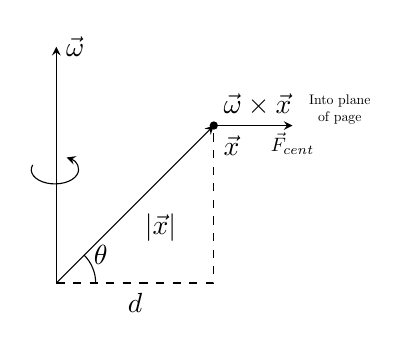
\begin{tikzpicture}[>=stealth]
  \draw[->] (0, 0)  -- (0, 3) node[right] {$\vec{\omega}$};
  \draw[->] (0, 0) -- (2, 2) node[below right] {$\vec{x}$} node[midway, below right] {$|\vec{x}|$};
  \fill (2, 2) circle (1.5pt) node[above right] {$\vec{\omega} \times \vec{x}$};
  \node[text width=2cm, align=center, scale=0.5] at (3.6, 2.2) {Into plane of page};
  \draw[->, yscale=0.6] (-0.3,2.5) arc [start angle=-200,end angle=60,radius=0.3];
  \draw (0.5,0) arc [start angle=0,end angle=45,radius=0.5] node[right] {$\theta$};
  \draw[dashed] (0, 0) -- (2, 0) node[midway, below] {$d$} -- (2, 2);

  \draw[->] (2, 2) -- (3, 2) node[below, scale=0.7] {$\vec{F}_{\text{cent}}$};
\end{tikzpicture}
\end{center}
The modulus of the centripetal force is:
\[
  |\vec{F}_{\text{cent}}| = m|\vec{\omega}||\vec{\omega} \times \vec{x}| = m\omega^2 r \sin\left(\frac{\pi}{2} - \theta\right) = m \omega^2 r \cos \theta
\]
It can also be written as the gradient of a scalar potential and so is a conservative force:
\[
  \vec{F}_{\text{cent}} = - \nabla V_{\text{cent}}
\]
where:
\[
  V_{\text{cent}} = - \frac{m}{2} |\vec{\omega} \times \vec{x}|^2 = - \frac{m}{2}\omega^2 r^2 \cos^2 \theta
\]
We can check this using suffix notation:
\begin{align*}
  [\nabla V_{\text{cent}}]_j &= -\frac{m}{2}\pderiv{}{x_j}([\vec{\omega} \times \vec{x}]_i[\vec{\omega} \times \vec{x}]_i) \\
                             &= -m [\vec{\omega} \times \vec{x}]_i \pderiv{}{x_j}(\levi_{i p q} \omega_p x_q) \\
                             &= -m [\vec{\omega} \times \vec{x}]_i \levi_{i p q} \omega_p \delta_{j q} \\
                             &= -m \levi_{i p j} [\vec{\omega} \times \vec{x}]_i \omega_p \\
                             &= -m [(\vec{\omega} \times \vec{x}) \times \vec{\omega}]_j
\end{align*}
Thus $\nabla V_{\text{cent}} = m \vec{\omega} \times (\vec{\omega} \times \vec{x})$ and so $\vec{F}_{\text{cent}} = -\nabla V_{\text{cent}}$.

As we move away from the axis of rotation, $r$ increases so the potential decreases as it becomes more negative.
\begin{example}
  Consider a string with a fixed mass $m$ hanging in equilibrium from it that is hanging from a fixed point above the surface of the Earth.
  \begin{center}
  \begin{tikzpicture}[>=stealth,decoration={
          markings,
          mark = at position 0.5 with {\arrow{>}}
        }]
    \begin{scope}
      \clip (0, 0) rectangle (3, 3);
      \draw (0, 0) circle (2);
    \end{scope}
    \draw (0, 0) -- (3.5, 3.5);
    \draw[postaction={decorate}] (2.8, 2) -- (3, 3) node[midway, right] {$\vec{T}$};
    \fill (2.8, 2) circle (1.5pt);
    \draw[->] (2.8, 2) -- (3.5, 2) node[midway, below right] {$\vec{F}_{\text{cent}}$};
    \draw[postaction={decorate}] (2.8, 2) -- (0, 0) node[midway, below] {$\vec{g}$};

    \draw[dashed] (0, 0) -- (2, 0) node[right, scale=0.6] {Equator};
    \draw (0, 0) ++ (0:0.6) arc (0:45:0.6) node[midway, right] {$\theta$};

    \draw (3, 3) ++ (-101:0.6) arc (-101:-135:0.6) node[midway, below left] {$\phi$};
  \end{tikzpicture}
  \end{center}
  Note that this diagram is very much \textbf{not to scale}.
  We want to find the angle $\phi$.

  We can ignore the Coriolis force here as the particle has no velocity, thus there are three forces acting on the particle: gravitational force, centripetal force, and tension from the string.

  It is most convenient if  we first find the radial and angular components of each of these forces in plane polar coordinates.


  Note that the string is very short compared to $R_{\text{Earth}}$ so it does not matter if take $\vec{r}$ at the top or at the bottom of the string and so we will use whichever is most convenient.

  The gravitational force $\vec{g}$ acts entirely radially and so:
  \[
    \vec{g} = - m g \uvec{r}
  \]
  To resolve the centripetal force, we see that:
  \begin{center}
  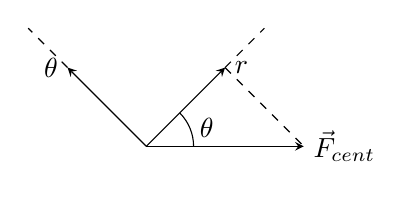
\begin{tikzpicture}[>=stealth]
    \draw[->] (0, 0)  -- (1, 1) node[right] {$\uvec{r}$};
    \draw[dashed] (1, 1)  -- (1.5, 1.5);
    \draw[->] (0, 0)  -- (-1, 1) node[left] {$\uvec{\theta}$};
    \draw[dashed] (-1, 1)  -- (-1.5, 1.5);
    \draw (0, 0) ++ (0:0.6) arc (0:45:0.6) node[midway, right] {$\theta$};
    \draw[->] (0, 0) -- (2, 0) node[right] {$\vec{F}_{\text{cent}}$};
    \draw[dashed] (1, 1) -- (2, 0);
  \end{tikzpicture}
  \end{center}
  So:
  \begin{align*}
    \vec{F}_{\text{cent}} &= -m \vec{\omega} \times (\vec{\omega} \times \vec{x}) \\
                          &= m \omega^2 r \cos \theta (\cos \theta \uvec{r} - \sin \theta \uvec{\theta})
  \end{align*}
  To hold the string together, there must be a force exerted by the molecules in the string that balances the other forces, this is called the \textit{tension} $\vec{T}$.
  We don't yet know $T = |\vec{T}|$ but we can still split $\vec{T}$ into radial and angular components.
  Noting that $\uvec{r}$ can be taken to the top of the string too, we see that:
  \begin{center}
  \begin{tikzpicture}[>=stealth]
    \draw[->] (0, 0)  -- (1, 1) node[right] {$\uvec{r}$};
    \draw[dashed] (1, 1)  -- (1.5, 1.5);
    \draw[->] (0, 0)  -- (-1, 1) node[left] {$\uvec{\theta}$};
    \draw[dashed] (-1, 1)  -- (-1.5, 1.5);
    \draw (0, 0) ++ (45:0.6) arc (45:64:0.6) node[midway, above right, scale=0.6] {$\phi$};

    \draw[dashed] (-0.5, -1) -- (0, 0);
    \draw[->] (0, 0) -- (1, 2) node[left] {$\vec{T}$};
    \draw[dashed] (1, 2) -- (1.5, 1.5);
  \end{tikzpicture}
  \end{center}
  and so:
  \[
    \vec{T} = T(\cos \phi \uvec{r} + \sin \phi \uvec{\theta})
  \]
  As the particle is in equilibrium, the sum of the forces will be $\vec{0}$ and so:
  \begin{align*}
    \vec{g} + \vec{F}_{\text{cent}} + \vec{T} = \vec{0}& \\
    \implies (-mg + m\omega^2 r \cos^2 \theta + T \cos \phi)\uvec{r} + (-m\omega^2 r \cos \theta \sin \theta + T\sin \phi) \uvec{\theta} = \vec{0}& \\
    \implies -mg + m \omega^2 r \cos^2 \theta + T \cos \phi = 0 \text{ and } -m\omega^2 r \cos \theta \sin \theta + T\sin \phi = 0& \\
    \implies T\cos \phi = m(g - \omega^2 r \cos^2 \theta) \text{ and } T \sin \phi = m\omega^2 r \cos \theta \sin \theta \\
    \implies \tan \phi = \frac{\omega^2 r \cos \theta \sin \theta}{g - \omega^2 r \cos^2 \theta}&
  \end{align*}
  At equator, we have $\theta = 0$ so $\phi = 0$, i.e. it hangs directly towards earth.
  When $\theta = \frac{\pi}{4}$, $\phi \approx \ang{e-4}$ so it is still a very small effect.
\end{example}
\section{Coriolis Force}
The Coriolis force is:
\[
  \vec{F}_{\text{cor}} = -2 m \vec{\omega} \times \vec{v}
\]
where $\vec{v}$ is the velocity in the rotating frame, i.e. $\left(\deriv{x}{t}\right)_{S'}$.
This is in the same form as the magnetic force from the Lorentz force (\cref{lorentzForce}) with $\vec{B} \mapsto \vec{\omega}$.
This means that moving particles will turn in circles as the force is always orthogonal to the direction of motion so makes the particle turn without changing its speed/doing work on the particle.

This makes sense as if a particle is not moving in an inertial frame, then it should be moving in a circle in a rotating frame and so the Coriolis force is the fictitious force responsible for this.
\begin{example}[Formation of Hurricanes]
  The Coriolis force is responsible for the formation of hurricanes.
  If a low pressure region forms in the atmosphere, particles will move in and so the Coriolis force ``bends'' their trajectory.

  Looking at earth from above the north pole, $-\vec{\omega}$ points into the plane of the page:
  \begin{center}
  \begin{tikzpicture}[>=stealth]
    \draw (0, 0) circle (3pt);

    \foreach \i in {0, 90, 180, 270} {
      \begin{scope}[rotate=\i]
        \draw[->] (1.5, 0) -- (0.3, 0);
        \draw[->] (0.9, 0.1) -- (0.9, 0.6);
      \end{scope}
    }

    \draw (-0.05, -0.05) -- (0.05, 0.05);
    \draw (-0.05, 0.05) -- (0.05, -0.05);
    \node[below right] {$-\vec{\omega}$};
  \end{tikzpicture}
  \end{center}
  The trajectory of each air molecule is bent clockwise (use right hand rule with $-\vec{\omega}$ going into the plane) and as we can see this leads to an anti-clockwise swirling motion.
  This means that hurricanes rotate anti-clockwise in the northern hemisphere and clockwise in the southern hemisphere.

  Near the equator $\vec{\omega} \times \vec{v}$, if motion is not equatorial, then it is not perpendicular to $\vec{\omega}$ and so is negligible, instead, if motion is along on the equator $\vec{\omega} \times \vec{v}$ can be substantive, however, we see that it pushes particles vertically and is negligible compared to gravity so can still usually be ignored.
  This is why we do not see hurricanes near the equator.
\end{example}
\begin{example}
  Suppose we drop a ball from rest at the top of a tower of height $h$ positioned on the equator.
  Where does the ball land?
  \begin{center}
  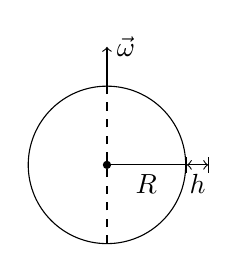
\begin{tikzpicture}
    \draw (0, 0) circle (1);
    \fill (0, 0) circle (1.5pt);
    \draw[->] (0, 1) -- (0, 1.5) node[right] {$\vec{\omega}$};
    \draw[dashed] (0, -1) -- (0, 1);
    \draw[-] (0, 0) -- (1, 0) node[midway, below] {$R$};
    \draw[|<->|] (1, 0) -- (1.3, 0) node[midway, below] {$h$};
  \end{tikzpicture}
  \end{center}
  Again this diagram is \textbf{not to scale}.

  \textbf{Using Angular Momentum in Inertial Frame}\par
  In the inertial frame, the only force is gravity, which is a central force so angular momentum of the ball $\ell$ is conserved.

  Initially $\ell = \omega(R + h)^2$, where $\omega$ is the angular speed of the Earth.
  At the floor of the tower $\ell = \omega'R^2$ where $\omega'$ is the angular speed of the ball around the Earth right before it hits the ground.
  Since angular momentum is conserve red $\omega(R + h)^2 = \omega'R^2$ and so $\omega' > \omega$.
  This means that the angular speed of the ball must increase as it falls in order to conserve $\ell$.
  So the ball must rotate faster than the tower and so will fall in front of the tower.

  \textbf{Using the Coriolis Force in Rotating Frame}\par
  In the rotating frame, we can neglect the centrifugal force because it is negligible near the equator.
  The equation of motion in the rotating frame is then:
  \[
    \ddot{\vec{x}} = \vec{g} - 2 \vec{\omega} \times \dot{\vec{x}}
  \]
  where $\vec{\omega}$ is the angular velocity of earth.

  Integrating, we have:
  \[
    \dot{\vec{x}} = \vec{g} t - 2 \vec{\omega} \times (\vec{x} - \vec{x}_0)
  \]
  Substituting back in:
  \[
    \ddot{\vec{x}} = \vec{g} - 2 \vec{\omega} \times \vec{g} t + 4 \vec{\omega} \times (\vec{\omega} \times (\vec{x} - \vec{x}_0))
  \]
  The final term can be neglected as it is of the same order as the centrifugal force, i.e. it acts in the vertical direction at the equator and is small compared to gravity.

  Thus:
  \[
    \ddot{\vec{x}} = \vec{g} - 2 \vec{\omega} \times \vec{g} t
  \]
  so integrating twice yields and using the initial condition that the ball is dropped from rest:
  \[
    \vec{x} = \vec{x}_0 +  \frac{1}{2}\vec{g} t^2 - \frac{1}{3} \vec{\omega} \times \vec{g} t^3
  \]

  We now define a right handed basis $\{\vec{e}_1, \vec{e}_2, \vec{e}_3\}$ where $\vec{e}_1$ points north, $\vec{e}_2$ points west and $\vec{e}_3$ points up the tower.
  This provides us with a basis local to the base of the tower in the rotating frame.

  We can express $\vec{\omega}$, $\vec{g}$ and $\vec{x}_0$ in this basis as:
  \[
    \vec{\omega} = \omega \vec{e}_1,\ \vec{g} = - g \vec{e}_3,\ \vec{x}_0 = (R + h)\vec{e}_3
  \]
  and so:
  \[
    \vec{x} = \begin{pmatrix}
    0 \\
    -\frac{1}{3}\omega g t^3 \\
    R + h - \frac{1}{2}gt^2 \\
    \end{pmatrix}
  \]
  The third component is just the standard equation of motion under gravity.
  We hit the ground when $\frac{1}{2}gt^2 = h$, and at this time, $-\frac{1}{3} \omega g t^3 < 0$ and so the ball lands to the east, in front of the tower.
\end{example}
\end{document}
